\documentclass[10pt]{beamer}
\usepackage[utf8]{inputenc}
\usepackage[T1]{fontenc}
\usepackage{lmodern}
\usepackage{amsmath}
\usepackage{cleveref}
\usepackage{amsfonts}
\usepackage{amssymb}
\usepackage{graphicx}
\newcommand{\pd}[2]{\frac{\partial{#1}}{\partial{#2}}}
\newcommand{\pdd}[2]{\frac{\partial^2{#1}}{\partial{#2}^2}}
\usepackage{optidef}
\usetheme{Warsaw}
\begin{document}
	\author{Mike Sutherland}
	\title{Surface Constraints for 3-D Path Planning}
	% \subtitle{}
	%\logo{}
	\institute{University of California, Irvine}
	\date{Nov 4, 2021}
	%\subject{}
	%\setbeamercovered{transparent}
	%\setbeamertemplate{navigation symbols}{}
	\begin{frame}[plain]
		\maketitle
	\end{frame}
	
	\begin{frame}
		\frametitle{We have a problem with planning in 3D.}
		\par 2.5D approaches: 
		\begin{itemize}
			\item "plane sandwich" approach
			\item when to hop planes?
			\item need to assess connectivity of each plane
			\item not optimal
		\end{itemize}
		\par Full 3D?
		\begin{itemize}
			\item Very expensive: A* on WxHxZ matrix?
			\item Other approaches (RRT, PRM, etc) can cut compute time... 
			\item ...but come with own downsides
			\item \textit{we want to spend most of the time close to the ground anyway}
		\end{itemize}
	\end{frame}

	\begin{frame}
		\textit{...we want to spend most of the time close to the ground anyway...} \\
		\bigskip
		Specifically:
		\bigskip
		\begin{itemize}
			\item at least some minimum distance off the ground
			\item at least some minimum distance from an obstacle
			\item not climbing too quickly
			\item not changing climb rate too quickly
		\end{itemize}
	\end{frame}

	\begin{frame}
	We can solve a convex problem
	
	\begin{mini!}|l|
		{h}{g(h) = h^2}
		{}{}
		\addConstraint{\pd{h}{\bar{x}} \leq h_{accel}\label{h_accel}}
		\addConstraint{\pdd{h}{\bar{x}} \leq h_{climb}\label{h_climb}}
		\addConstraint{h \geq h_{min}\label{hmin}}
		\addConstraint{h \geq h_{obs} + h_{barrier}\label{h_barrier}}
		\addConstraint{\bar{x} \in (\mathcal{X, Y})\label{xy}}
	\end{mini!}
	This optimization produces a mapping, $h$, for every $\bar{x} \in (\mathcal{X, Y})$, which corresponds to the "sheet" of possible positions for the aircraft.
	\end{frame}

	\begin{frame}
		\frametitle{What does this look like?}

		\begin{figure}
			\centering
			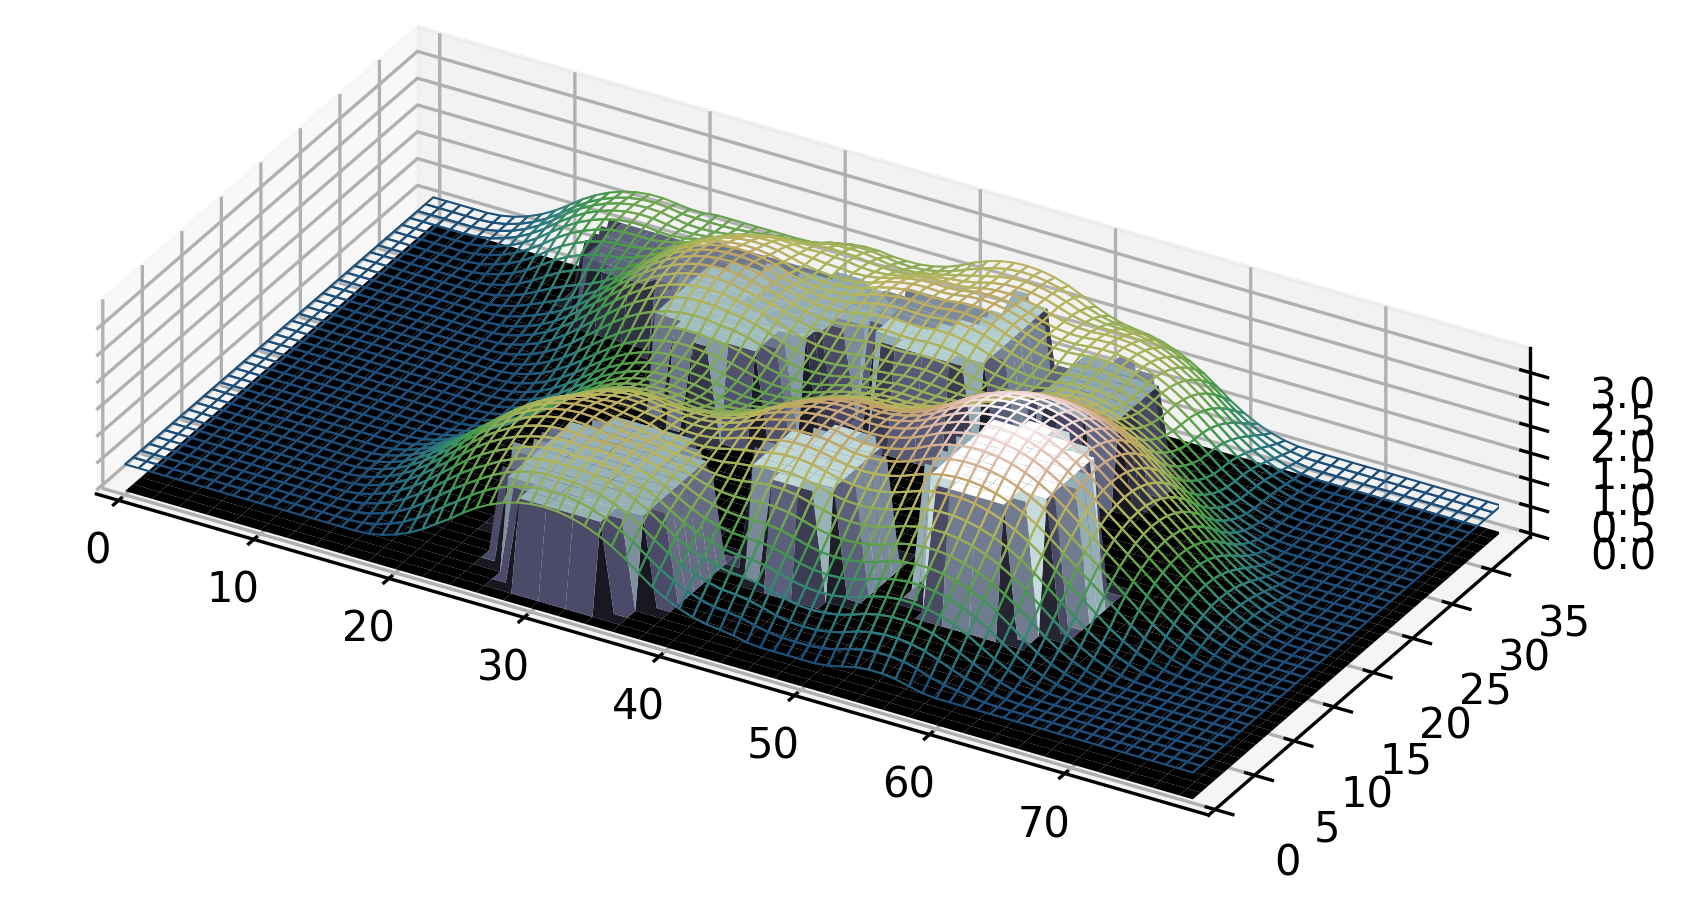
\includegraphics[width=0.7\linewidth]{astar-3d.png}
			\caption{The mesh created by solving the optimization problem. We have an area of obstacles, each with a height. The solution is a mapping from $\mathcal{(X, Y)} \rightarrow H$, which is shown here in 3-d by the wireframe. The surface is smooth and as low as possible without hitting the obstacles.}
			\label{fig:mesh}
		\end{figure}
		
	\end{frame}

	\begin{frame}
		\frametitle{Runtime}
		We are solving an optimization problem over a mesh. So, runtime is roughly quadratic.
		
		\begin{figure}
			\centering
			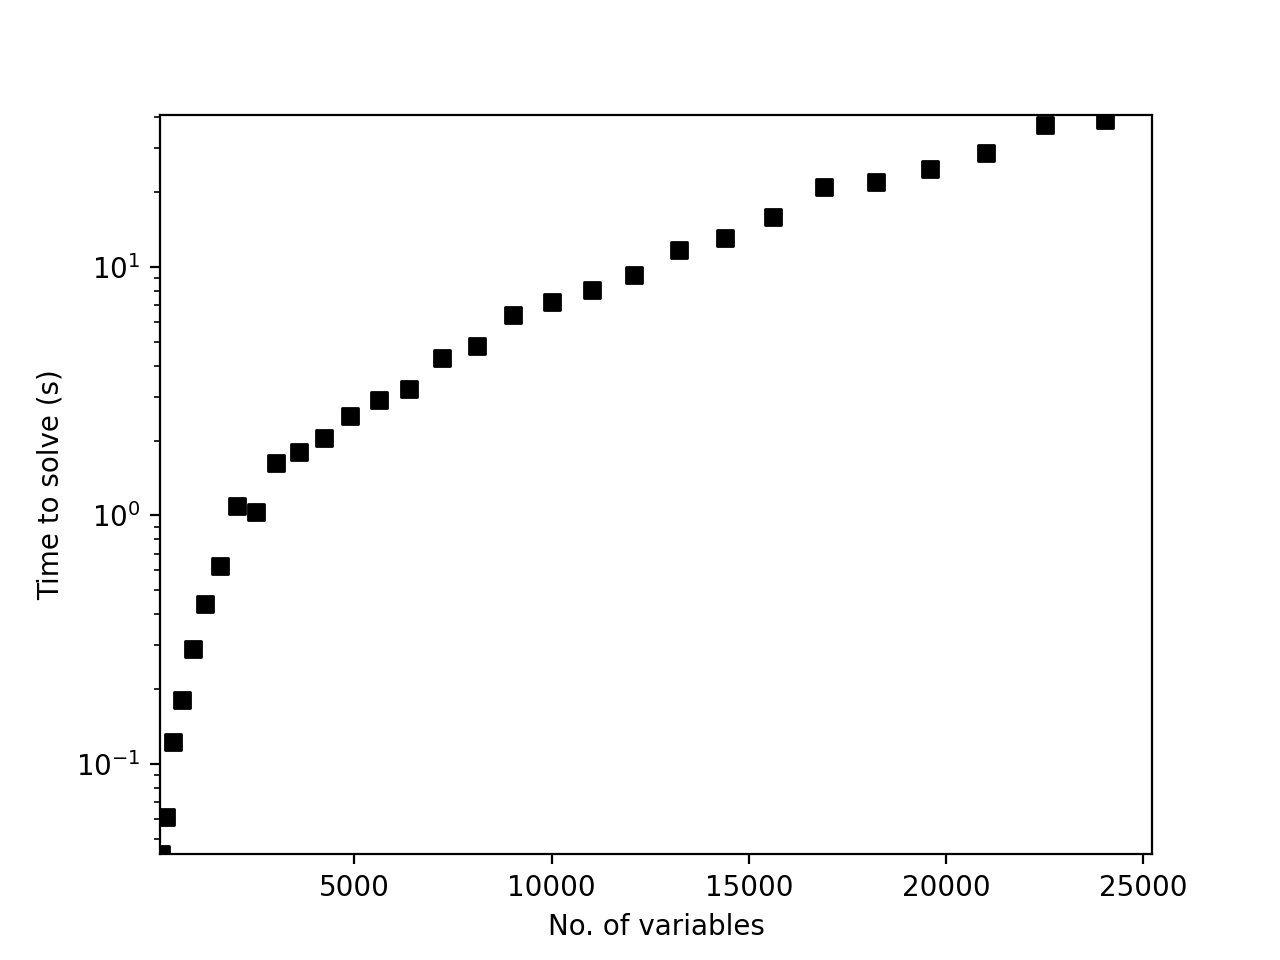
\includegraphics[width=0.6\linewidth]{speed}
			\caption{Runtime of the algorithm. Each grid point counts as a variable, and grid ponts scale roughly linearly with area, assuming an equal distance between points.}
			\label{fig:speed}
		\end{figure}
		
		
		
	\end{frame}

	\begin{frame}
		\frametitle{Now, how to plan?}
		\begin{itemize}
			\item Planners such as A* and derivatives, RRT, PRM, and so on can be used in $\mathbb{R}^2$ as normal
			\item If desired, cost heuristics that use the mapping can be used to weight the path to be lower or higher.
			\item We lose 1 degree of freedom when re-planning around dynamic obstacles; for example, we cannot fly below or above the sheet to move around obstacles.
			\item Collisions with dynamic objects can be cheaply calculated in $\mathbb{R}^2$ if necessary.
			\item For dynamic objects, spherical collisions are cheap for the sheet.
		\end{itemize}
	\end{frame}	
	
	\begin{frame}
		\begin{figure}
		\centering
		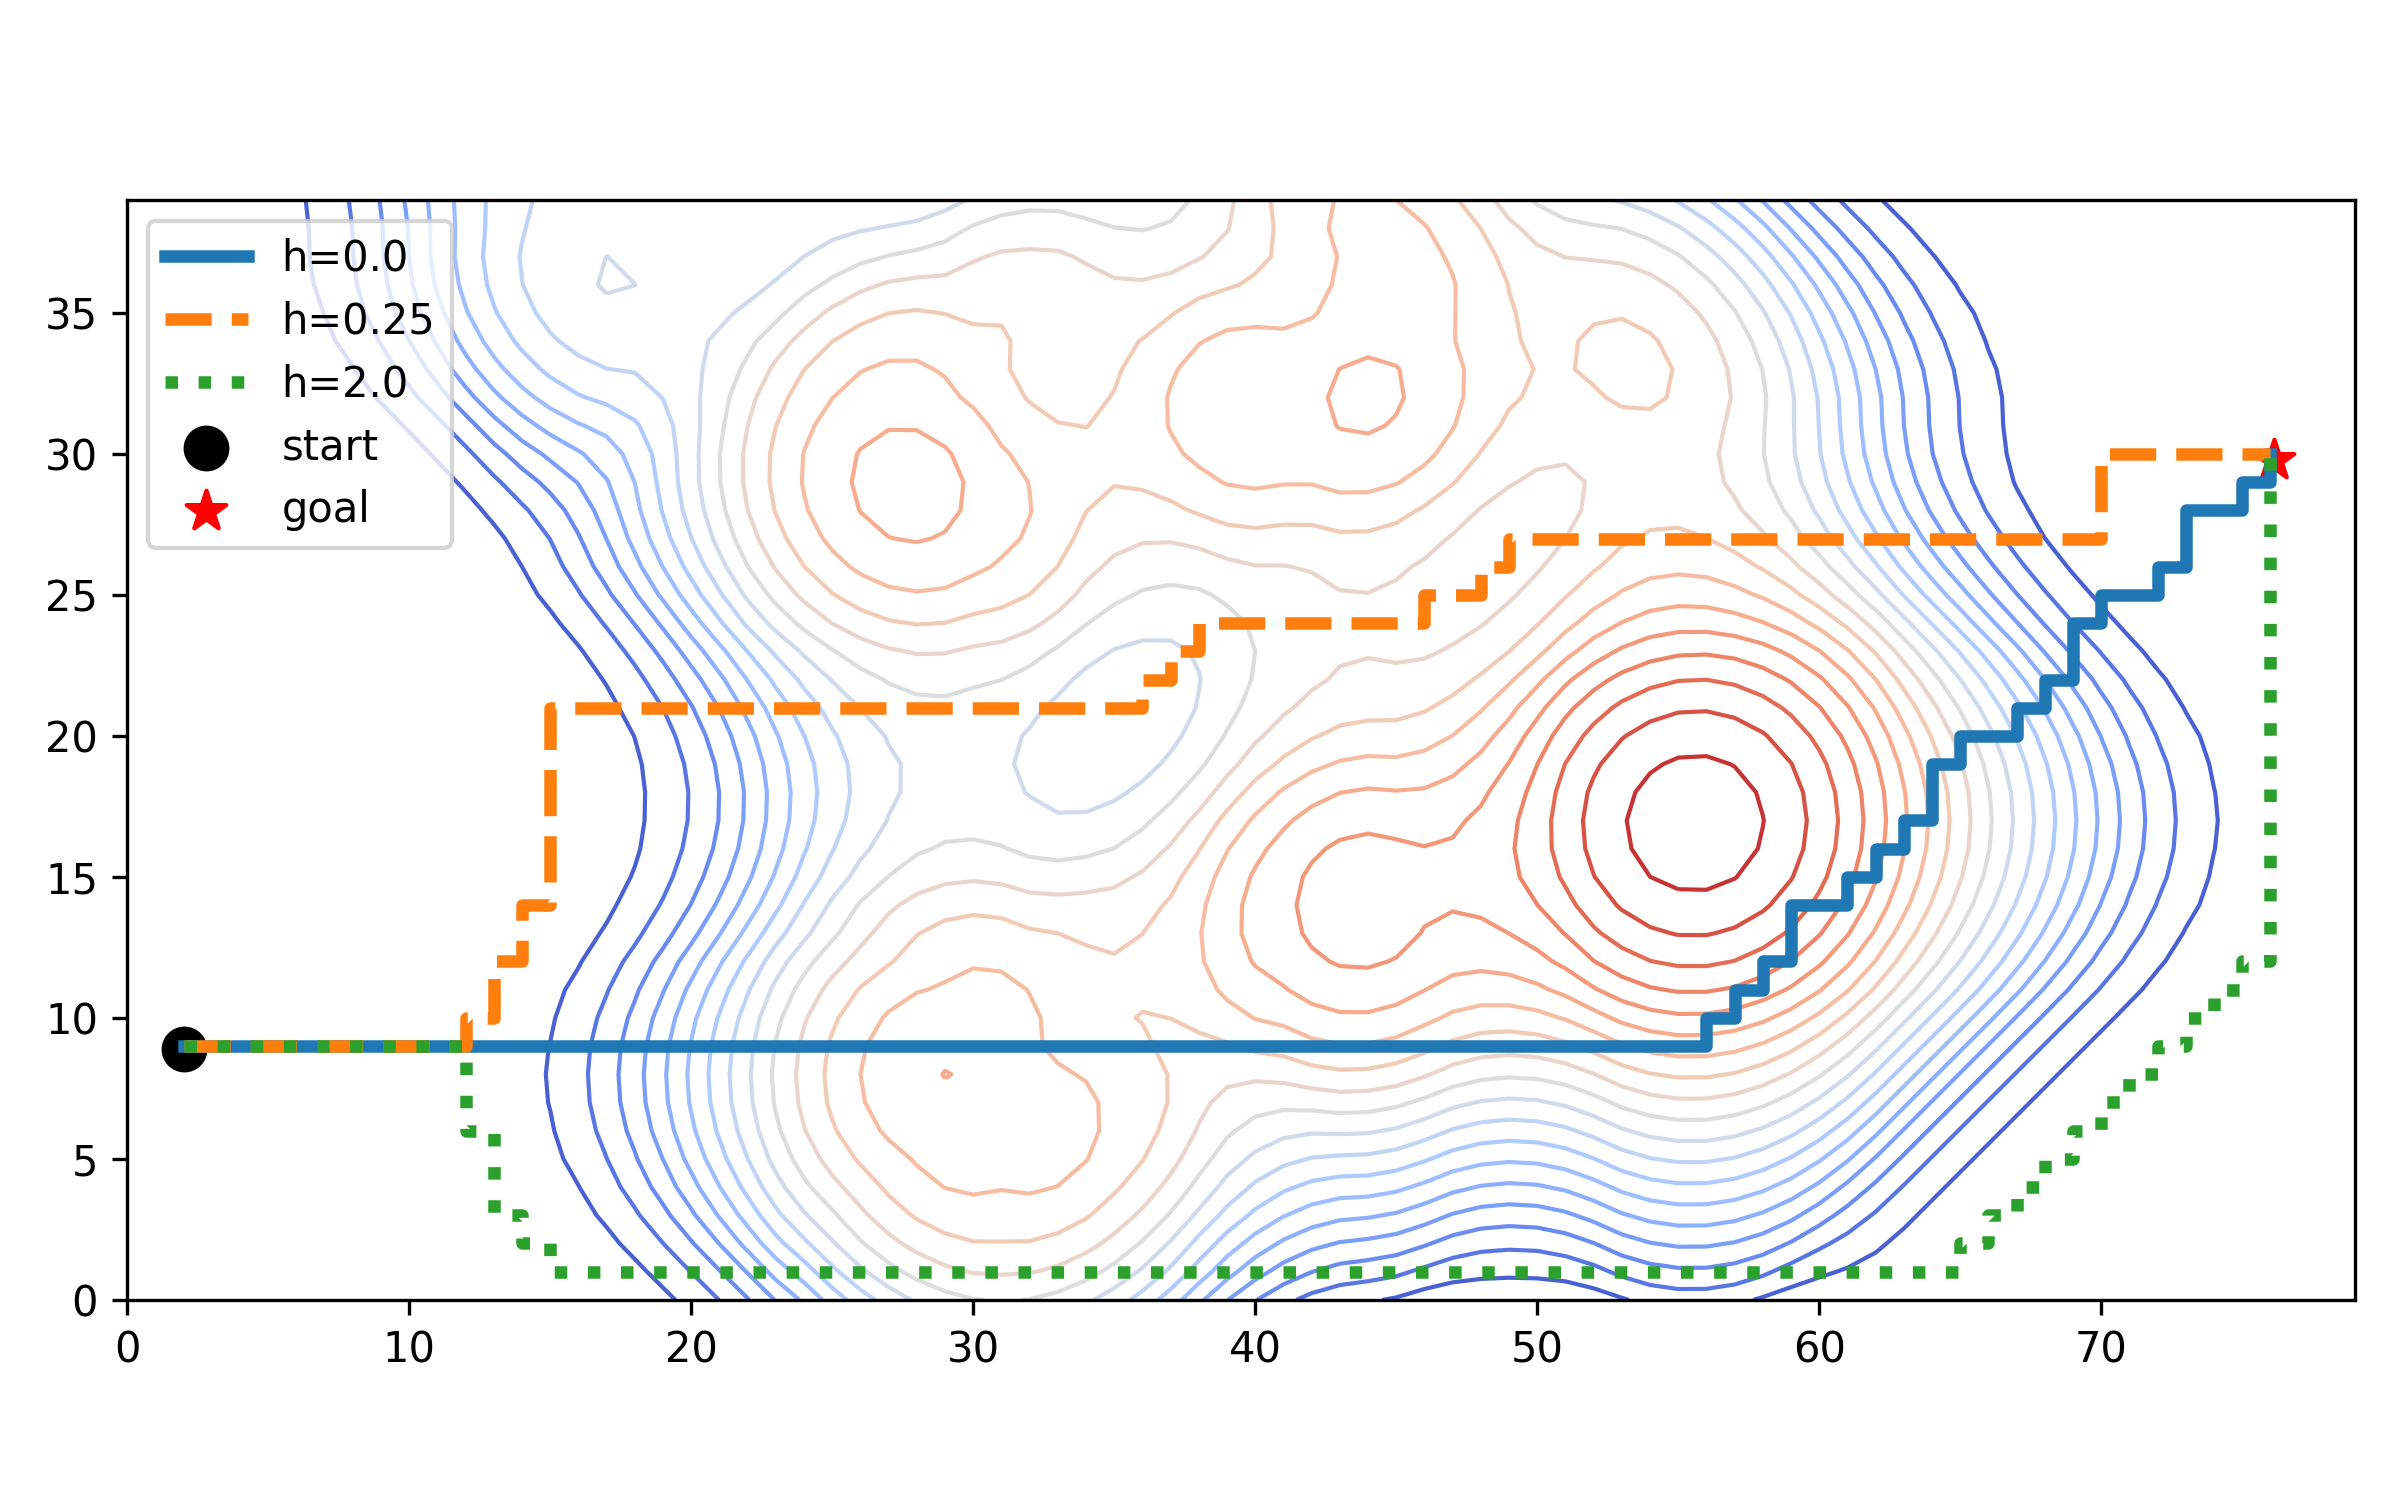
\includegraphics[width=.8\linewidth]{astar-2d.png}
		\caption[Different weights of $h$ in the A* planner.]{A standard A* planner moves from one point to another through a field of obstacles (the same field as \cref{fig:mesh}). A different cost weight is applied on $h$. When $h$ is higher, the planner strongly penalizes $h$, whereas when $h$ is lower, the planner does not care about $h$ as much. All paths, however, are tractable within the vehicle dynamics and collision constraints.}
		\label{fig:hcost}
		\end{figure}
	\end{frame}

	\begin{frame}
		\frametitle{Next Steps}
		\begin{itemize}
			\item Dynamic sampling density: more points sampled near obstacles
			\item Explore cost heuristics in algorithms (and make some proofs?)
			\item Boundary conditions with $h_{obs} = \infty$ obstacles
			\item Speed up optimization?
		\end{itemize}
	\end{frame}

\end{document}